\chapter{実験}
本章では,提案する視覚エフェクトと振動刺激の提示手法を用いた評価実験を行った.
本章では実験内容及びその結果を示す.

評価実験では,VR上に魔法の杖を表示しそこから特定の形状の魔法を放つ.
それに伴い,ユーザーに対しさまざまな振動刺激を与える.
これにより魔法の形状に対してどのような振動刺激をユーザーに与えることで,ユーザーの魔法体験感を高めることができるのかを調査する.

\section{実験方法}
本章では作成したシステムを用いた評価実験を行った.
22歳$\sim$24歳の男性8名に対して実験を実施した.

本実験の手順を以下に示す.
手順の2$\sim$4の工程をinceneration,ring-fire,main-beamの順番にそれぞれ繰り返す.
被験者は振動を体験してもらった後,アンケートに回答してもらうので振動パターンを覚えておく必要がある.
その旨を実験説明の段階で被験者に伝える.

\begin{enumerate}
    \item 実験説明
    \item 実験前アンケート
    \item 実験
    \item 実験後アンケート
\end{enumerate}

\newpage
\section{実験前アンケート}
実験を実施する前にアンケートを行う.

まず,被験者に実験で使用する視覚エフェクトの動画を見せる.
次に視覚エフェクトを時系列順に6分割し並べた画像を被験者に見せる.
それぞれ振動強度がどのように変化しそうであるか,被験者のイメージを手書きでグラフに書いてもらった.
振動強度のグラフを\figref{ank}に示す.

ユーザーが視覚エフェクトに対してどのような振動刺激が与えられるとイメージしているのかを調査する.

\begin{figure}[h]
\centering
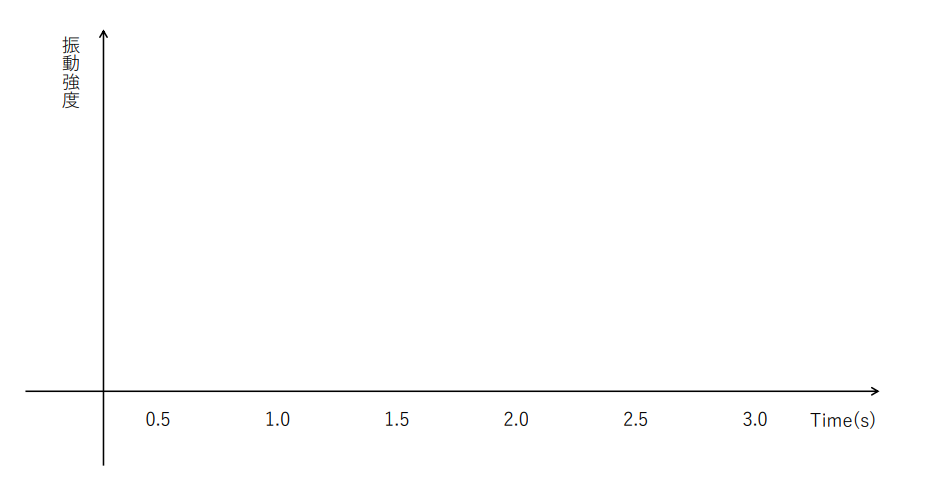
\includegraphics[clip,width=10cm]{./fig/ank.png}
\caption{振動強度のイメージ}\label{ank}
\end{figure}

\section{実験}
被験者はHMDを装着し右手にコントローラーを持つ.
実験の様子を\figref{jikken}に,実験の被験者の視界を\figref{first}に示す.
提示する視覚エフェクトと振動パターンを実験者が選択する.
この時被験者に選択したエフェクトを伝えておく.
視覚エフェクトに対して4パターンの振動刺激を提示した後アンケートを実施する.
これを視覚エフェクトの種類ごとに繰り返す.


実験終了後にアンケートを行う.
実験終了後アンケートでは視覚エフェクトに対しての振動刺激の一致度を5段階で評価してもらった.
システム使用中の没入感やその他気になったことや感想は自由記入形式で回答してもらった.
\begin{figure}[h]
\centering
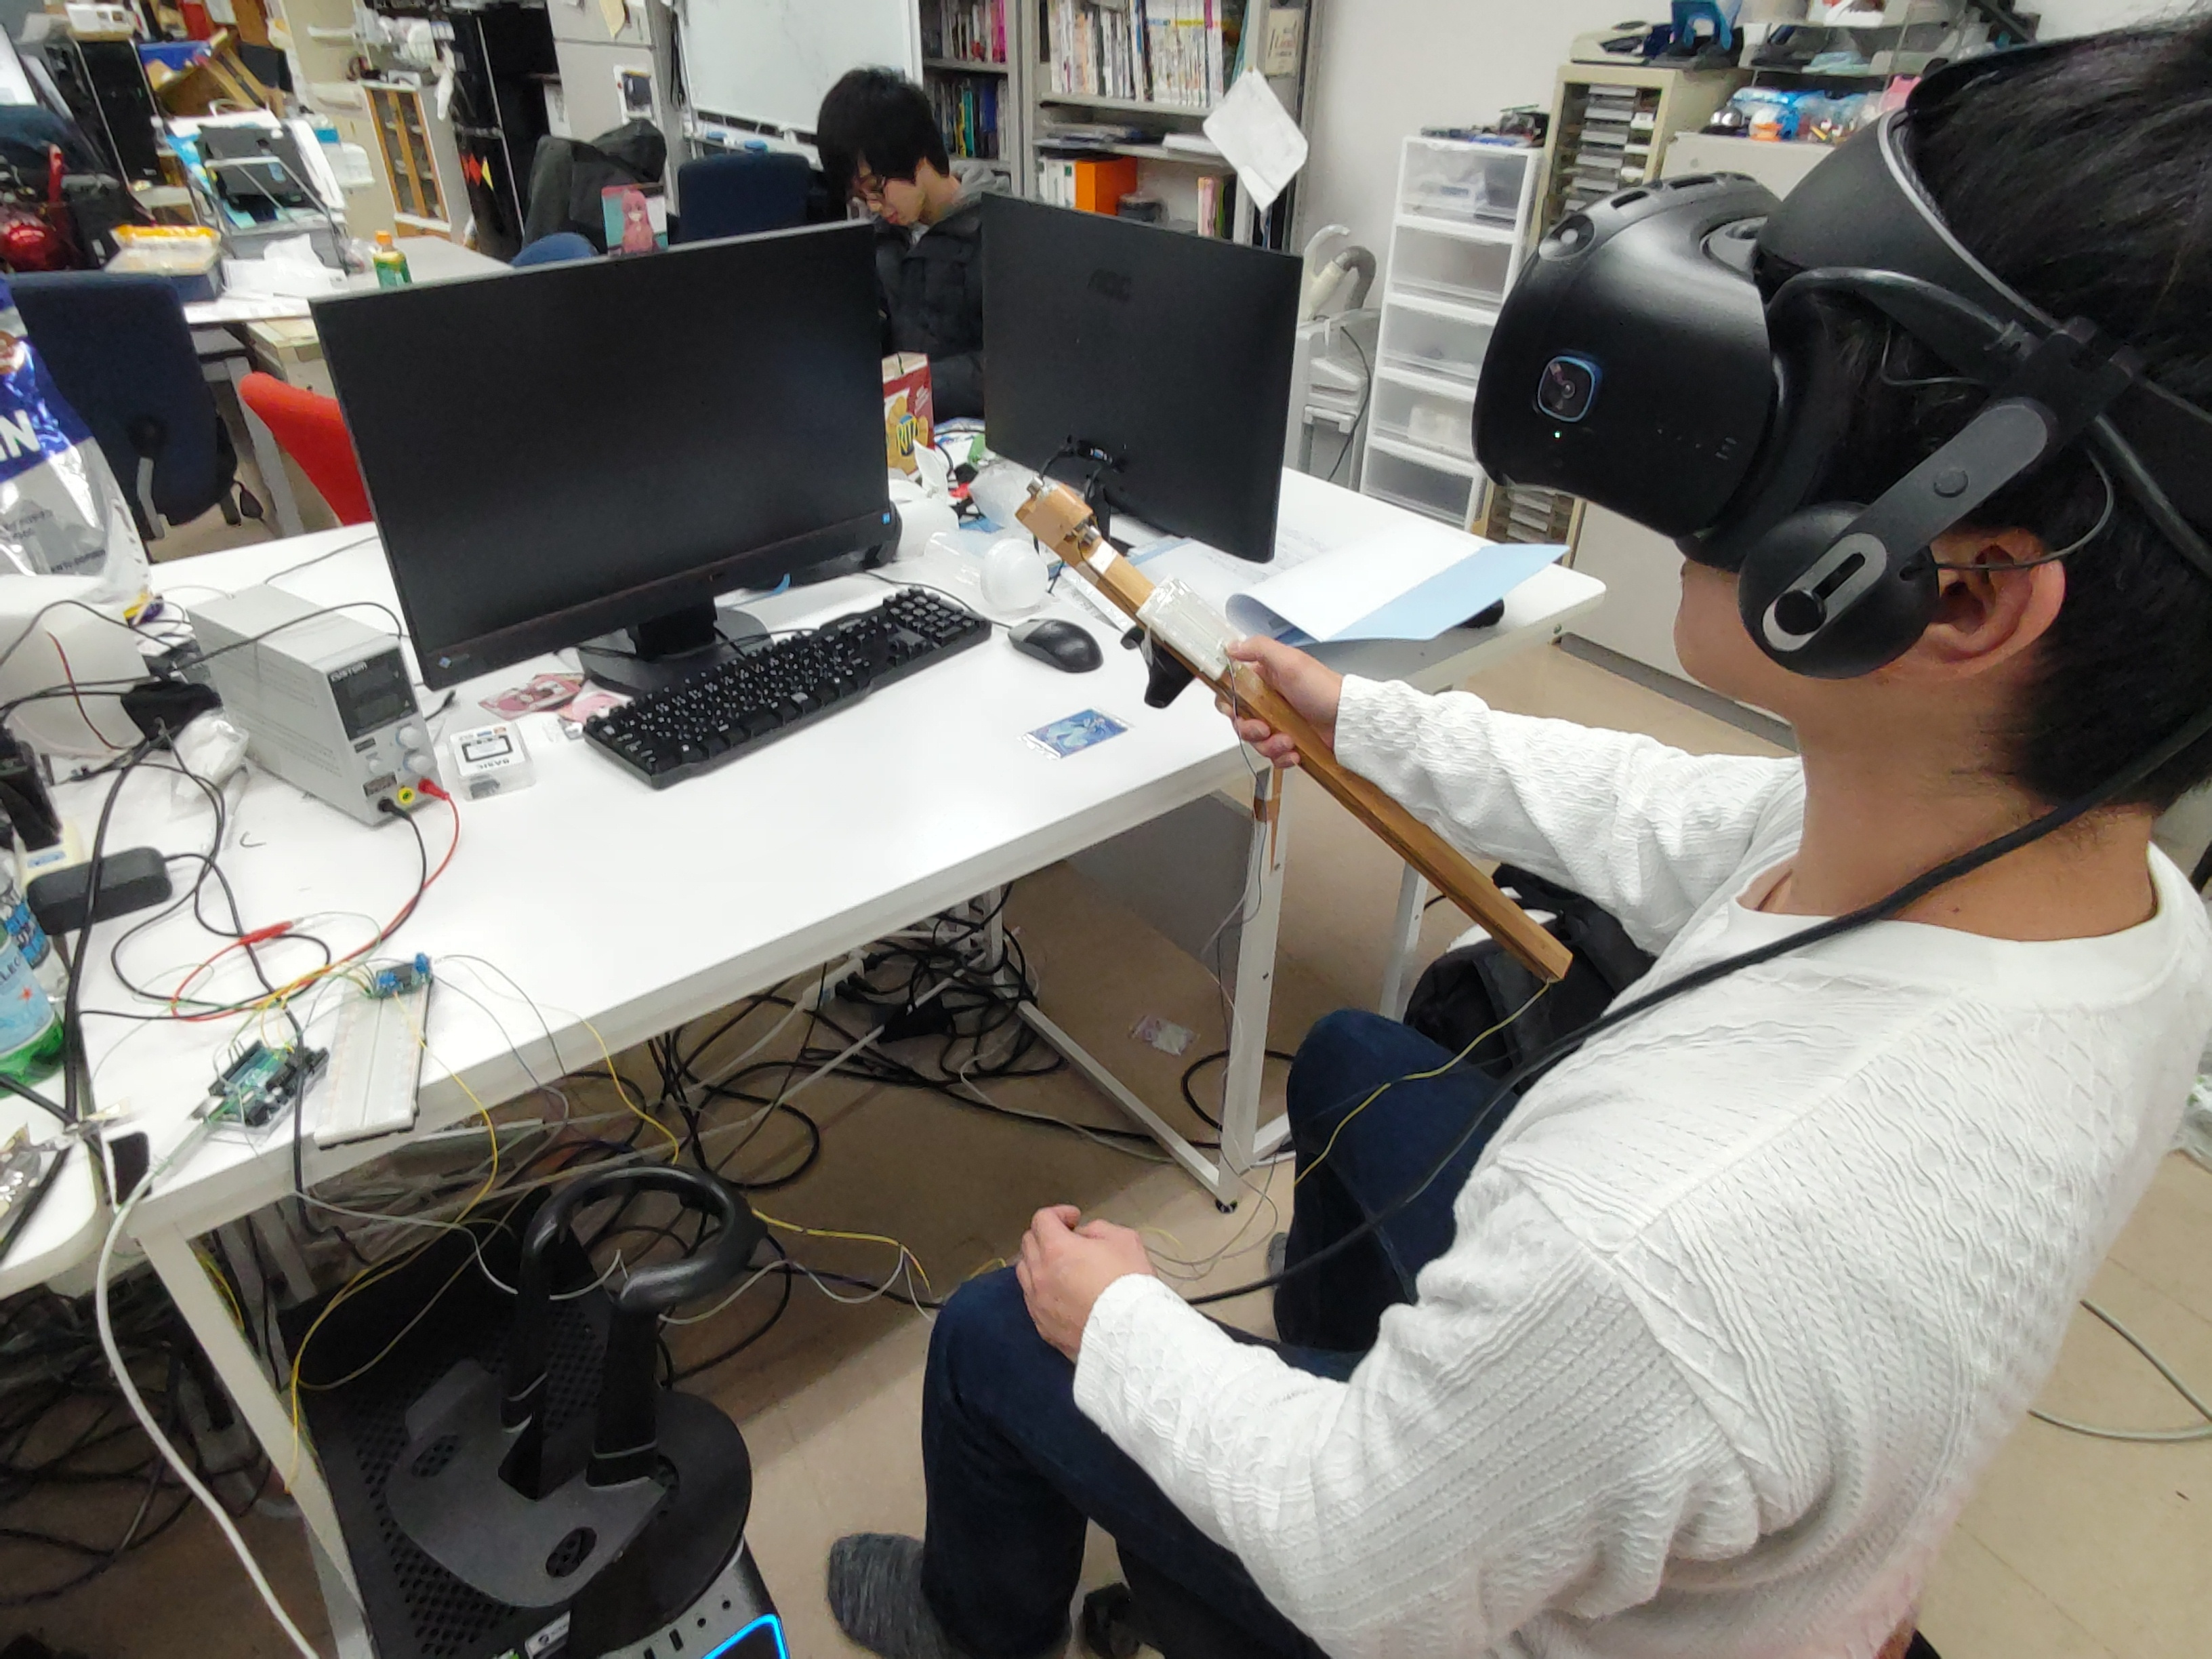
\includegraphics[clip,width=10cm]{./fig/jikken.png}
\caption{実験の様子}\label{jikken}
\end{figure}
\begin{figure}[h]
\centering
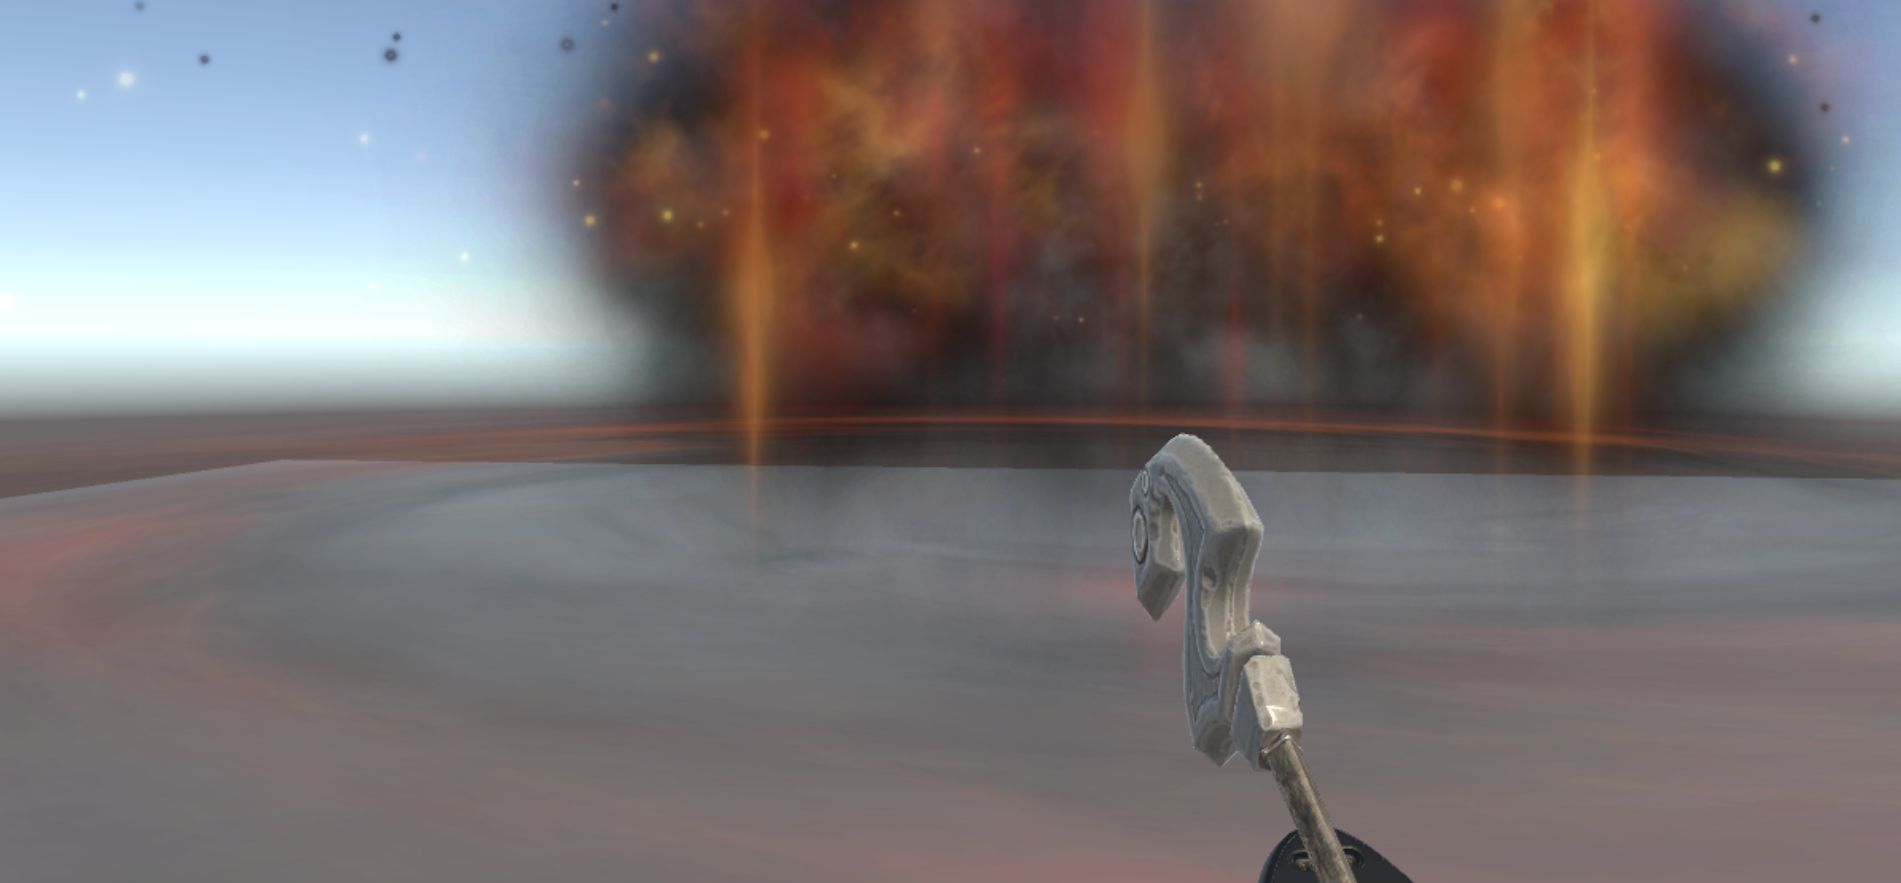
\includegraphics[clip,width=10cm]{./fig/unity.png}
\caption{被験者の視界}\label{first}
\end{figure}

\newpage

\section{結果と考察}
\subsection{実験前アンケート結果}
以下に実験前アンケートの結果を示す.
\figref{inceA}にincenerationについてのアンケート結果を示す.
被験者ほぼ全員がincenerationの振動について,一定であると回答した.
振動パターン1に近い結果となった.
\begin{figure}[h]
\centering
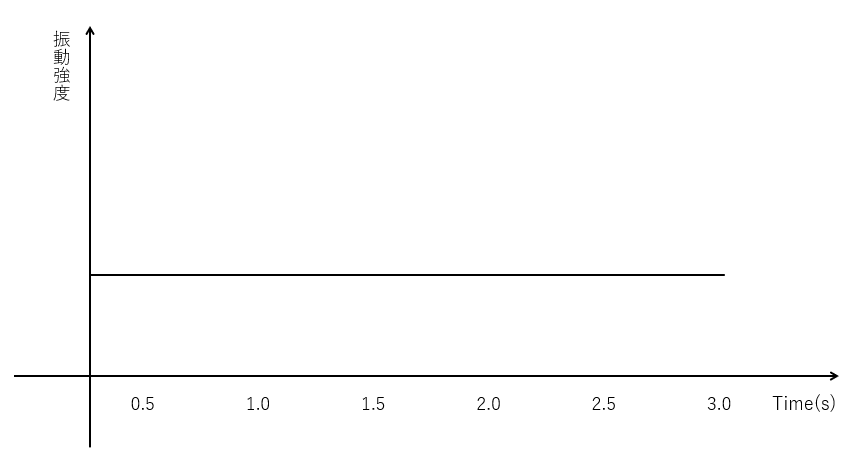
\includegraphics[clip,width=8cm]{fig/incenerationAve.png}
\caption{アンケート結果(inceneration)}\label{inceA}
\end{figure}


\figref{ringA}にring-fireについてのアンケート結果を示す.
2枚目までは小さい振動が続き,3枚目で大きな振動になり,残りは余韻といったイメージであることが分かる.
振動パターン2に近い結果となった.
\begin{figure}[h]
\centering
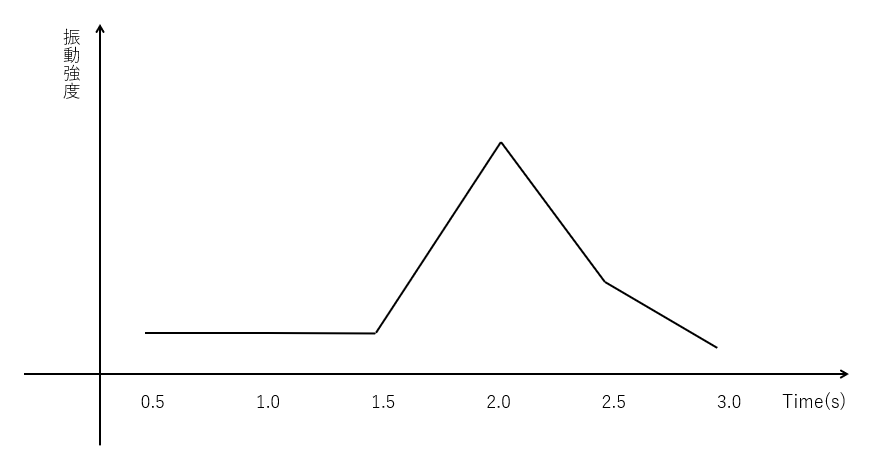
\includegraphics[clip,width=8cm]{fig/ringfireAve.png}
\caption{アンケート結果(ring-fire)}\label{ringA}
\end{figure}



\figref{mainA}にmain-beamについてのアンケート結果を示す.
ring-fireと比較して初めから強い振動があり,残りは余韻といったイメージであることが分かる.
振動パターン3に近い結果となった.
\begin{figure}[h]
\centering
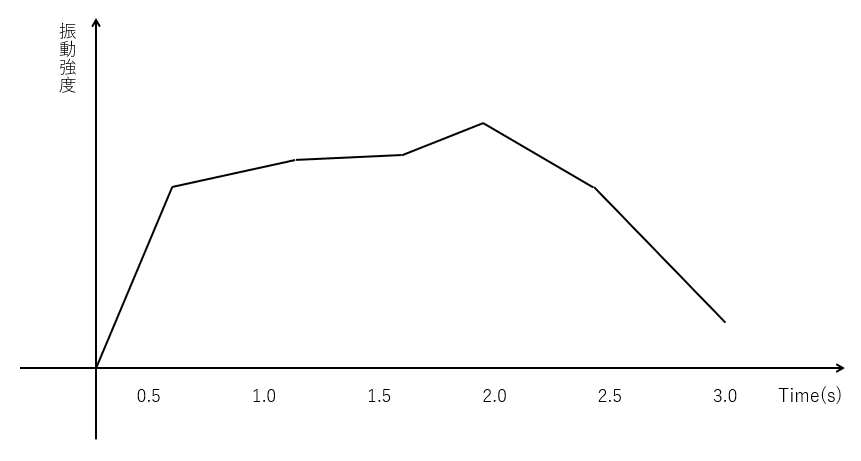
\includegraphics[clip,width=8cm]{fig/mainbeamAve.png}
\caption{アンケート結果(main-beam)}\label{mainA}
\end{figure}

\newpage

\subsection{実験後アンケート結果}
アンケート結果の5段階評価の平均を求める.

平均=(評価の数値×人数)のパターン1からパターン4までの合計÷被験者数とする.

\figref{inceAnk}にinceneration体験後のアンケートを示す.

\begin{figure}[h]
  \centering
  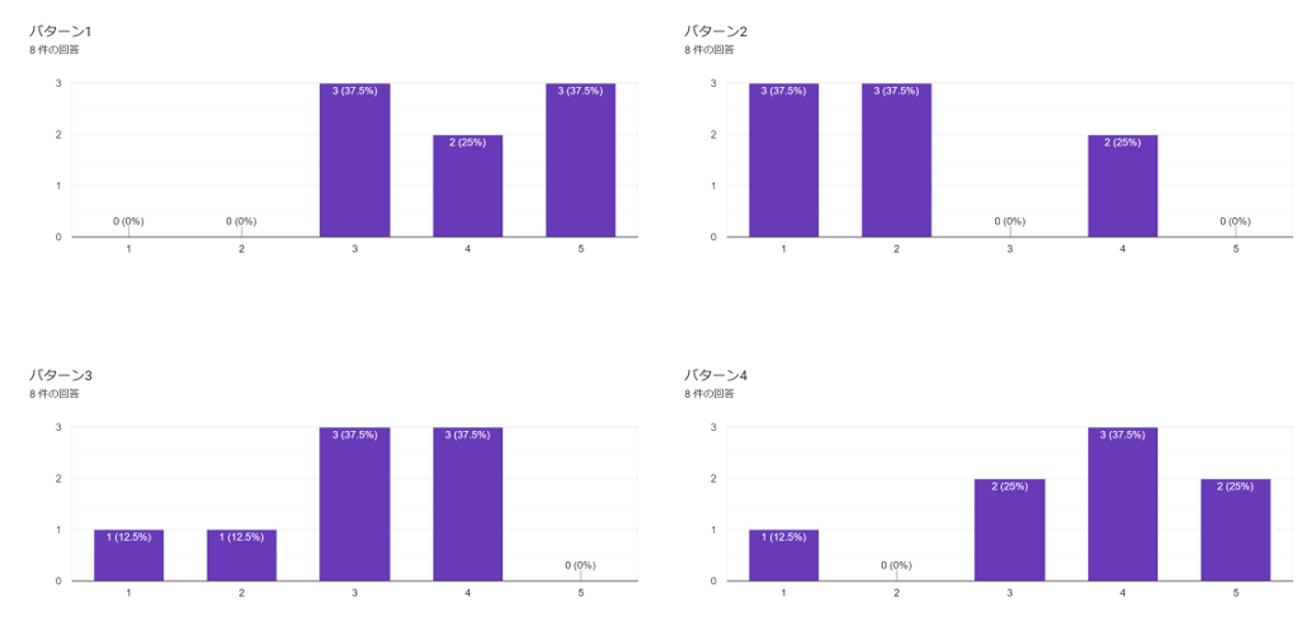
\includegraphics[clip,width=14cm]{./fig/incenerationAnk.png}
  \caption{アンケート結果(inceneration)}\label{inceAnk}
  \end{figure}
  


平均値を\tabref{tab;inceAvera}に示す.
これよりパターン1とパターン4の評価が高くなっている.
実験前アンケートと比較すると,実験者のイメージと同じ振動刺激を与えると没入感を高められることが分かる.
\begin{table}[h]
    \caption{平均値(inceneration)}
    \centering
    \begin{tabular}{l|l}
    \hline
    \hline
    パターン1 & 4\\
    パターン2 & 2.125\\
    パターン3 & 3\\
    パターン4 & 3.625\\
    \hline
    \end{tabular}
    \label{tab;inceAvera}
\end{table}

\figref{ringAnk}にring-fire体験後のアンケートを示す.

\begin{figure}[h]
  \centering
  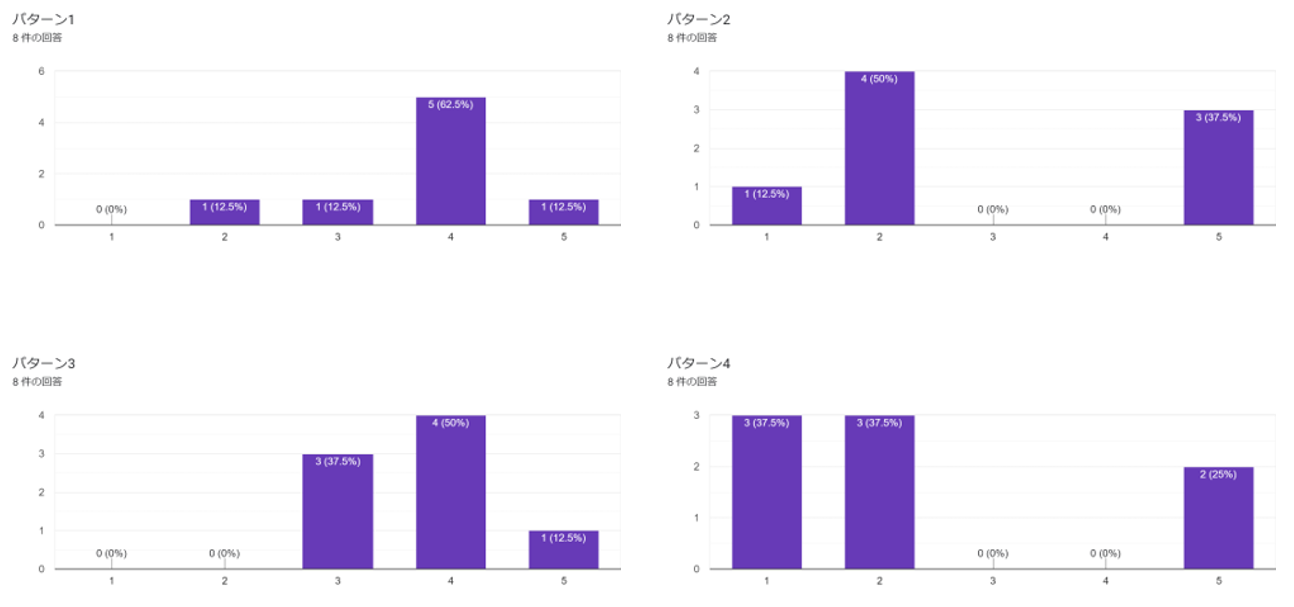
\includegraphics[clip,width=14cm]{fig/ringfireAnk.png}
  \caption{アンケート結果(ring-fire)}\label{ringAnk}
  \end{figure}


平均値を\tabref{tab;ringAve}に示す.
パターン2の平均値が3.875と高くなっている.
これは後から爆発が起こるという実験前アンケートの結果と一致していると言える.

\begin{table}[h]
    \caption{平均値(ring-fire)}
    \centering
    \begin{tabular}{l|l}
    \hline
    \hline
    パターン1 & 3.75\\
    パターン2 & 3\\
    パターン3 & 3.75\\
    パターン4 & 2.375\\
    \hline
    \end{tabular}
    \label{tab;ringAve}
\end{table}

\figref{mainAnk}にmain-beam体験後のアンケート結果を示す.

\begin{figure}[h]
  \centering
  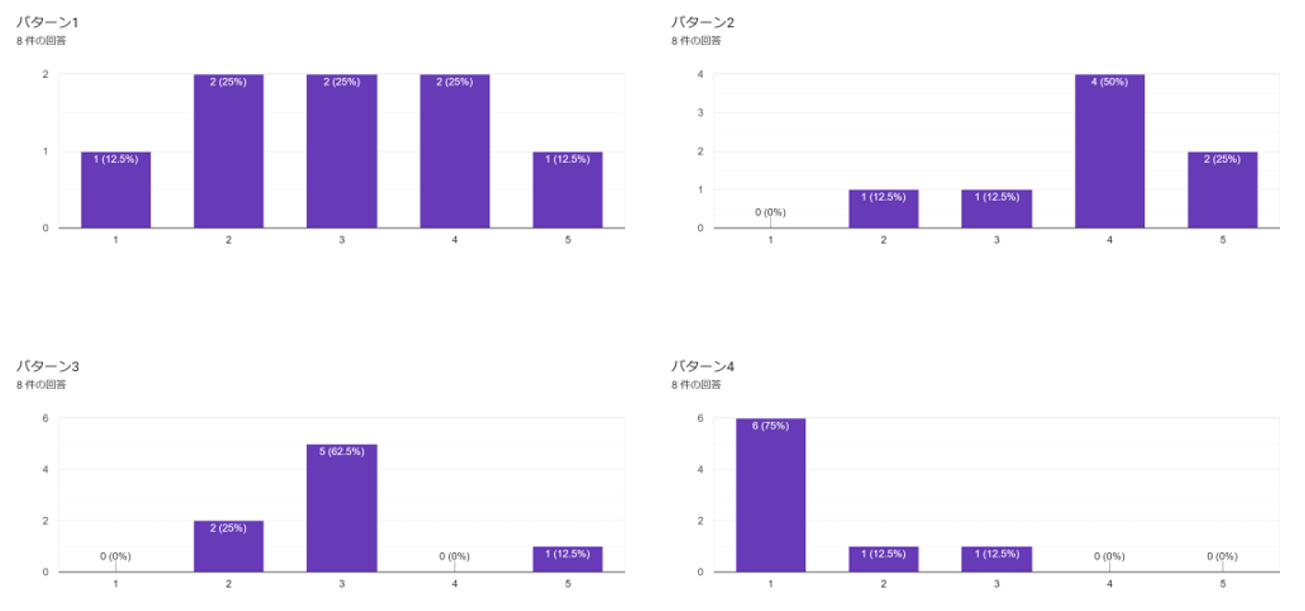
\includegraphics[clip,width=14cm]{fig/mainbeamAnk.png}
  \caption{アンケート結果(main-beam)}\label{mainAnk}
  \end{figure}


平均値を\tabref{tab;mainAve}に示す.
パターン1とパターン3の評価が高くなっている.
実験前アンケートの初めに大きい振動が来てその後余韻が残るという結果に沿っている.

  \begin{table}[H]
    \caption{平均値(main-beam)}
    \centering
    \begin{tabular}{l|l}
    \hline
    \hline
    パターン1 & 3\\
    パターン2 & 3.875\\
    パターン3 & 3\\
    パターン4 & 1.375\\
    \hline
    \end{tabular}
    \label{tab;mainAve}
\end{table}

事前アンケートの結果と同じような波形の振動パターンの評価が高くなる傾向にあった.

視覚エフェクトが大きくなるタイミングで振動も大きくなると視覚エフェクトと振動刺激が一致していると感じる傾向にある.


